\documentclass{article}

% if you need to pass options to natbib, use, e.g.:
% \PassOptionsToPackage{numbers, compress}{natbib}
% before loading nips_2016
%
% to avoid loading the natbib package, add option nonatbib:
% \usepackage[nonatbib]{nips_2016}

%\usepackage{nips_2016}

% to compile a camera-ready version, add the [final] option, e.g.:
\usepackage[final]{nips_2016}

\usepackage[utf8]{inputenc} % allow utf-8 input
\usepackage[T1]{fontenc}    % use 8-bit T1 fonts
\usepackage{hyperref}       % hyperlinks
\usepackage{url}            % simple URL typesetting
\usepackage{booktabs}       % professional-quality tables
\usepackage{amsfonts}       % blackboard math symbols
\usepackage{nicefrac}       % compact symbols for 1/2, etc.
\usepackage{microtype}      % microtypography




\usepackage[style=numeric,backend=bibtex,maxbibnames=99]{biblatex}
\addbibresource{references.bib}

\usepackage{graphicx}
\usepackage{caption}
\usepackage{subcaption}
\usepackage{float}
\usepackage{amsmath,amsfonts,amsthm,bm} % Math packages

\graphicspath{{img/}} %Setting the graphicspath




\title{Removing Noise from Speech with Deep Learning}

% The \author macro works with any number of authors. There are two
% commands used to separate the names and addresses of multiple
% authors: \And and \AND.
%
% Using \And between authors leaves it to LaTeX to determine where to
% break the lines. Using \AND forces a line break at that point. So,
% if LaTeX puts 3 of 4 authors names on the first line, and the last
% on the second line, try using \AND instead of \And before the third
% author name.

\author{
	Glávits Balázs \\
	Department of Measurement and Information Systems\\
	Budapest University of Technology and Economics\\
	\texttt{email@email.email} \\
	 \And
	Kiss Andor \\
	Department of Automation and Applied Informatics\\
	Budapest University of Technology and Economics\\
	\texttt{email@email.email} \\	 
	 \And
	Konrád Márk \\
	Department of Telecommunications and Media Informatics\\
	Budapest University of Technology and Economics\\
	\texttt{konrad0816@gmail.com} \\
	%% \AND
	%% Coauthor \\
	%% Affiliation \\
	%% Address \\
	%% \texttt{email} \\
	%% \And
	%% Coauthor \\
	%% Affiliation \\
	%% Address \\
	%% \texttt{email} \\
	%% \And
	%% Coauthor \\
	%% Affiliation \\
	%% Address \\
	%% \texttt{email} \\
}

\begin{document}
	% \nipsfinalcopy is no longer used
	
	\maketitle
	
	\begin{abstract}
		TODO
	\end{abstract}
	\newpage
	\section{Task summary}
		Our goal is to reduce (or in the best case, entirely remove) the noise from audio recordings containing noisy speech. The idea is to use the WaveNet\cite{wavenet}\cite{dataset} architecture to generate clean audio from the noisy one.
	\section{Data acquisition and exploration}
	For our training and testing data, we used a dataset called "\href{https://datashare.is.ed.ac.uk/handle/10283/2791}{Noisy speech database for training speech enhancement algorithms and TTS models}"\cite{dataset} by the University of Edinburgh. It consists of $\sim$23000 clean-noisy pairs (figure \ref{fig:clean_noisy_noise}) from 56 different speakers. 
	The samples are stored in separate .wav files of varying length (figure \ref{fig:dur}).  

	\begin{figure}[H]
		\centering
		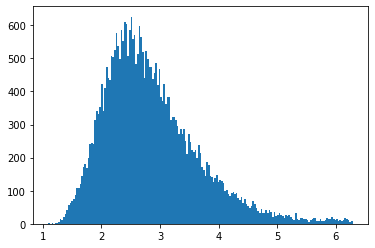
\includegraphics[width=.5\linewidth]{durations}
		\caption{Duration distribution histogram of a subset of speeches}
		\label{fig:dur}
	\end{figure}

	\begin{figure}[H]
		\centering
		\begin{subfigure}{.5\textwidth}
			\centering
			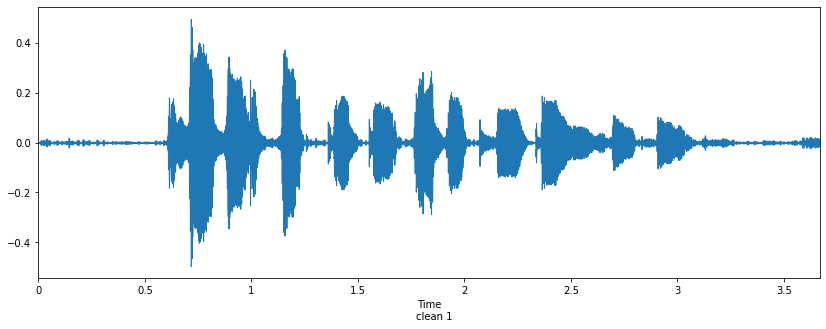
\includegraphics[width=.8\linewidth]{wave_for_noise_clean}
			\caption{clean}
			\label{fig:wave_for_noise_clean}
		\end{subfigure}%
		\begin{subfigure}{.5\textwidth}
			\centering
			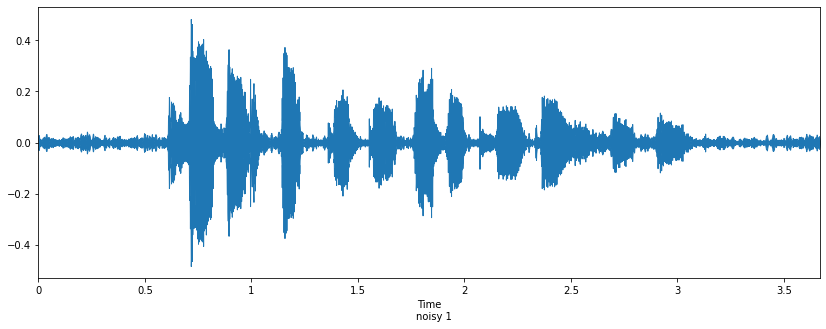
\includegraphics[width=.8\linewidth]{wave_for_noise_noisy}
			\caption{noisy}
			\label{fig:wave_for_noise_noisy}
		\end{subfigure}
		\label{fig:clean_noisy_n}
		
		\begin{subfigure}{.7\textwidth}
			\centering
			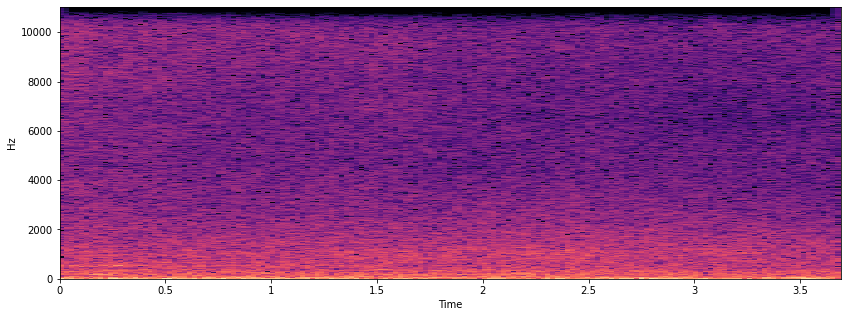
\includegraphics[width=.8\linewidth]{noise}
			\caption{noise spectogram}
			\label{fig:noise}
		\end{subfigure}
		\caption{Noisy and clean samples and the spectogram of the noise from the audio in figures \ref{fig:wave_for_noise_clean} and \ref{fig:wave_for_noise_noisy}}
		\label{fig:clean_noisy_noise}
	\end{figure}

	

	\section{Data preprocessing}

	Our first approach was to select the $n$ closest audio samples and zero-pad them to be the same duration, then reduce the samples to 8 bit with $\mu$-law transformation (figure \ref{fig:clean_noisy_padded_mulaw}).
	
	\begin{figure}[H]
		\centering
		\begin{subfigure}{.5\textwidth}
			\centering
			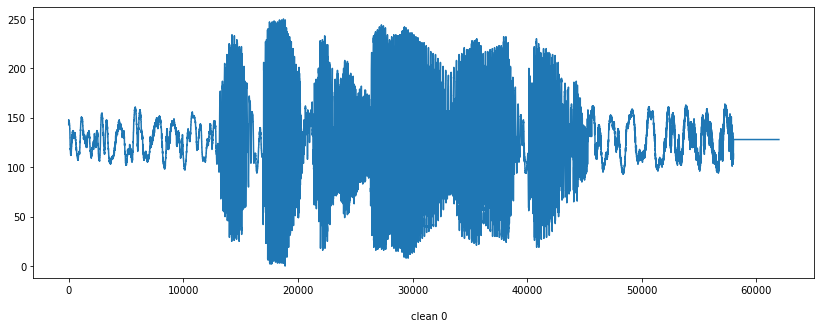
\includegraphics[width=.8\linewidth]{wave_clean_padded_mulaw}
			\caption{clean}
			\label{fig:wave_clean_padded_mulaw}
		\end{subfigure}%
		\begin{subfigure}{.5\textwidth}
			\centering
			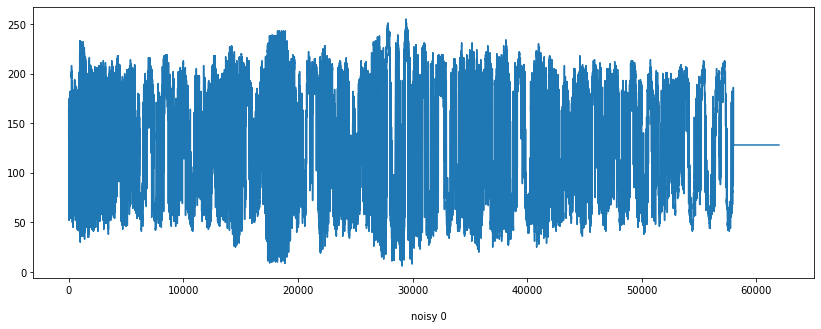
\includegraphics[width=.8\linewidth]{wave_noisy_padded_mulaw}
			\caption{noisy}
			\label{fig:wave_noisy_padded_mulaw}
		\end{subfigure}
		\caption{An example clean-noisy pair after padding and $\mu$-law transformation}
		\label{fig:clean_noisy_padded_mulaw}
	\end{figure}
	
	With this implementation we ran into the problem of limited hardware resources so, we had to come up with a less resource-intensive preprocessing pipeline.
	
	Our solution was to load the raw data, normalize it between -1 and 1 and downsample it to 16kHz. After these preprocessing steps, we feed the audio to the model with a data generator which can generate batches of smaller same sized pieces of data.
	With this approach, we eliminated the memory problem but sacrificed some of the continuity in our speech samples. The other upside of this solution is that we don't have to feed the meaningless data to the model in the form of zeroes.
	
	The original implementation of the WaveNet architecture used one-hot encoded $\mu$-law transformed data, but after experimenting with these, we could not generate audio with acceptable quality.


	\section{The WaveNet architecture}
	For our network architecture, we choose to use a modified version of the WaveNet\cite{wavenet} architecture developed by DeepMind.

	WaveNet is a deep neural network capable of generating raw audio waveforms. This can be achieved with the use of a dilated causal convolutional layers. Causal means that the network is only conditioned on past and current inputs. With this approach, we can make sure that the ordering of the data is not violated. With dilation, we can achieve a large receptive field with the preservation of the input resolution. The structure of a stack created with these kinds of layers can be seen in figure \ref{fig:dccs}.
	
		
	\begin{figure}[H]
		\centering
		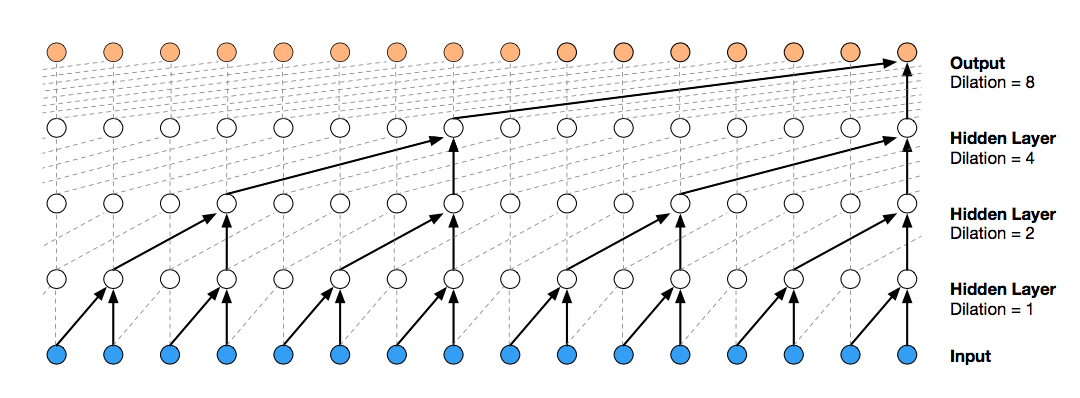
\includegraphics[width=.8\linewidth]{dccs.png}
		\caption{A dilated causal convolutional layer stack}
		\label{fig:dccs}
	\end{figure}
	
	The model uses residual blocks and skip connections to speed up the convergence and enable the use of deeper networks.
	
	\begin{figure}[H]
		\centering
		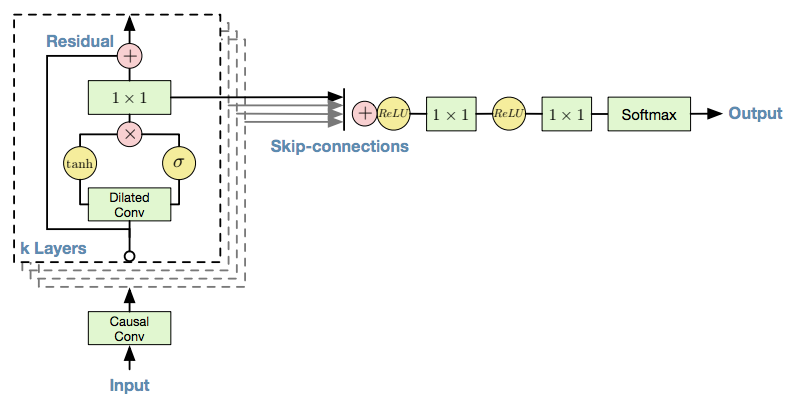
\includegraphics[width=.8\linewidth]{residual.png}
		\caption{Residual blocks in WaveNet}
		\label{fig:residual}
	\end{figure}
	
	\subsection{WaveNet for noise removing}
	
	\subsection{Our denoising WaveNet implementation}
	
	
	\newpage
	\printbibliography



\end{document}